La progettazione dell'interfaccia grafica e dell'esperienza utente (UX) è una fase cruciale nella realizzazione di un software di successo. Nel contesto dell'obiettivo di questa tesi, che mira a facilitare i dipendenti dell'Azienda X nel raggiungimento dei loro luoghi di lavoro, questa Sezione descrive le scelte di progettazione che hanno contribuito a creare un'interfaccia utente più intuitiva, attraverso un'esperienza di utilizzo migliorata della mappa di ZConnect.

La progettazione dell'interfaccia grafica e dell'UX è stata guidata dalla necessità di fornire ai dipendenti un accesso rapido e intuitivo alle informazioni necessarie per raggiungere i loro luoghi di lavoro e registrare le presenze. L'ottimizzazione di funzionalità chiave, come la visualizzazione della posizione corrente dell'utente e dei luoghi di lavoro associati, nonché l'introduzione di nuove caratteristiche, come il "follow-me", hanno contribuito in modo significativo al raggiungimento di questi obiettivi.

\section{Progettazione delle interfacce grafiche e della UX}\label{Progettazione}
La progettazione dell'interfaccia grafica e dell'esperienza utente (UX) costituisce un elemento significativo all'interno di questo lavoro di tesi. L'obiettivo fondamentale di questa fase è stato progettare sistemi in grado di agevolare i dipendenti dell'Azienda X nel raggiungimento dei luoghi di lavoro. Per conseguire tale scopo, è stato necessario rivisitare l'interfaccia grafica dell'applicazione ZConnect.

Come riportato nella Sezione \ref{Problemi_sistema} nell'implementazione precedente a questo lavoro di tesi, il servizio di monitoraggio delle presenze di ZConnect non forniva un supporto adeguato agli utenti nel raggiungimento dell'area di lavoro. Per risolvere questo problema, è stata progettata la mappa in modo che mostri chiaramente la posizione dell'utente e l'area di lavoro da raggiungere.

Inoltre, come riportato nella Sezione \ref{Analisi_sistema} del capitolo di Analisi, ad ogni utente di ZConnect è associata una lista di luoghi geografici, modellati come geofence, in cui l'utente può effettuare la timbratura. Data questa molteplicità di luoghi in cui l'utente può registrare la propria presenza, è stato progettato di visualizzarli tutti sulla mappa, contrariamente a quanto avveniva prima dell'intervento descritto in questa tesi, come visibile in Figura \ref{fig:tanti_geofence}. In modo tale da agevolare l'utente nel raggiungimento del luogo di lavoro corretto, infatti essendo associati all'utente numerosi luoghi geografici non è possibile sapere a priori quale è quello in cui l'utente deve recarsi, di conseguenza non è plausibile scegliere un solo luogo da mostrare all'utente sulla mappa, scartando gli altri.

\begin{figure}[ht!]
    \centering
    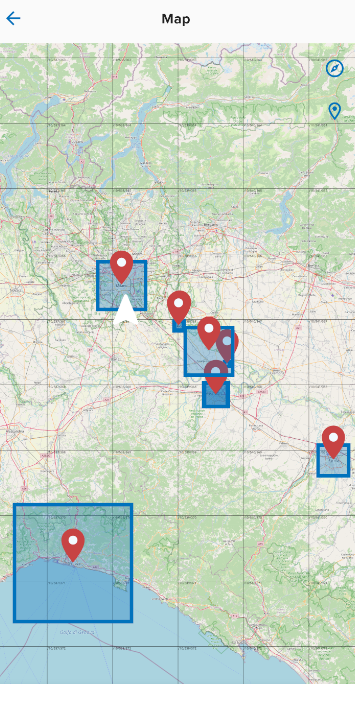
\includegraphics[width=0.4\textwidth]{Immagini/tanti_geofence.png}
    \caption{Mappa di un utente con tanti geofence}
    \label{fig:tanti_geofence}
\end{figure}

Al fine di garantire un'esperienza utente ottimale, è stato ritenuto essenziale rendere chiaramente visibili all'utente, all'apertura della mappa, la propria posizione e il luogo di lavoro da raggiungere. Per questo motivo, è stata adottata l'opzione di centrare la mappa sulla posizione attuale dell'utente all'apertura della stessa. Inoltre, è stato impostato un adeguato livello di zoom della mappa per consentire all'utente di visualizzare contemporaneamente la propria posizione e il centro del luogo di lavoro più vicino. Un esempio di zoom della mappa alla sua apertura è visibile in Figura \ref{fig:zoom_vicino}, in cui sono chiaramente visibili la posizione dell'utente e il luogo di lavoro più vicino

\begin{figure}[ht!]
    \centering
    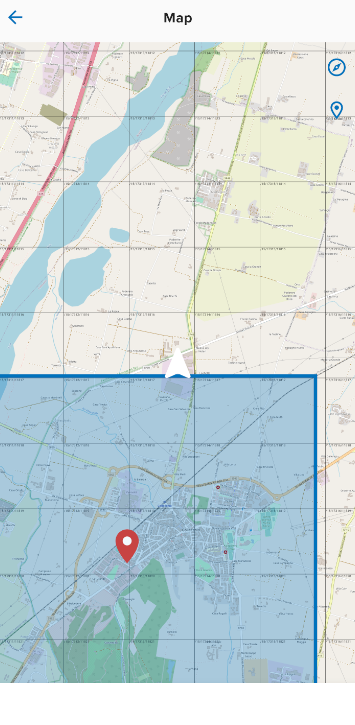
\includegraphics[width=0.4\textwidth]{Immagini/zoom_vicino.png}
    \caption{Zoom della mappa all'apertura}
    \label{fig:zoom_vicino}
\end{figure}

Questa scelta è stata motivata dall'ipotesi che, in un caso d'uso normale, l'utente non utilizzi questa mappa come navigatore e, pertanto, non dovrebbe aprirla quando si trova a grandi distanze dal luogo di lavoro. Si è ipotizzato che l'utente debba aprire la mappa solamente in prossimità del luogo di lavoro per comprendere la relazione tra la sua posizione e il luogo di lavoro, utilizzando la mappa come supporto per raggiungere il luogo dove registrare la propria presenza. Pertanto, si è ritenuto che fosse efficace per l'utente visualizzare la sua posizione e il luogo di lavoro più vicino al fine di orientarsi facilmente.

Durante la fase di progettazione dell'interfaccia grafica, si è valutato che la mappa dovesse fornire degli strumenti che agevolassero l'utente nel suo utilizzo. Per fare questo, è stata implementata una funzionalità di "follow-me", attivabile tramite un bottone sulla schermata della mappa. All'attivazione della funzionalità di "follow-me", la mappa scorre automaticamente, seguendo lo spostamento dell'utente, e rimane centrata sulla posizione dell'utente. Questa funzionalità agevola la navigazione dell'utente nello spazio che lo circonda, perché, nello spostamento per raggiungere il luogo di lavoro, non deve continuamente interagire con la mappa per vedere la sua posizione su di essa.

Inoltre, è stata considerata l'aggiunta di un bottone che permette all'utente di centrare la mappa sulla sua posizione corrente, in modo che anche se dovesse interagire con la mappa togliendo dal focus il marker con la sua posizione, non perda contezza di dove è la sua posizione, ma con un click la ritrovi immediatamente.

